\subsection{Data Understanding}

In this chapter, the collected data is analyzed in detail.
This process starts at the data source, meaning how and why spotify collects the data.
Then the features, the Spotify algorithm uses, are covered in detail.
This includes a theoretical explanation of each feature and its format and numerical representation.
The most important features are finally compared visually using appropriate graphs and plots.

\subsubsection{The Streaming Service Spotify}
%Spotify is a music streaming service and has established itself as the Number one in this market. 
%Since their launch in 2006, the company has gained over \(365\) million users, of which nearly \(45\) percent
%are subscribed to the chargeable premium service. 
%This Premium service comes at a subscription cost of nowadays \(12,99\)€ per month,
%giving the opportunity to listen to every song that is available at Spotify - this being
%ca. \(70\) million tracks from over \(1,2\) million Artists. \cite[]{L.Rabe2021}
As stated in the introduction, Spotify is the leading streaming service.
Their extensive catalogue of about \(70\) million tracks from over \(1,2\) million Artists
necessitates Spotify to focus on Big Data Analytics to generate business value and a competitive advantage.
The main objective here is to understand the music itself and their user's behavior and interests,
in order to offer personalized recommendations and curated playlists.
The company evaluates millions of songs and and uses AI to independently recognize
patterns and structures within different genres. 
A good example for personalized content is the "Discover Weekly" playlist, which recommends 30 new songs
to each user on a weekly basis. 

At the moment, the Spotify algorithm, which goes by the name Echo Nest,
consists of three main components \cite{Stephenson2021}.
First of all, it creates an individual taste profile for each individual user. 
Data is collected about which artists, songs, albums, playlists, podcast and audio books the
respective user listens to. The listening duration, frequency and listening location is also recorded.
Different users can then be compared against each other using these metrics, to find matching 
taste profiles among them.
For example, if \emph{user a} has a large overlap in musical taste with \emph{user b}'s playlists,
songs from \emph{user b}'s playlists will end up in \emph{a}'s weekly recommendation.
Furthermore, popular playlists with a large amount of followers are considered more often for recommendation puposes \cite[]{Stephenson2021}.

In addition, the algorithm analyzes the individual components of the music itself. 
It breaks down each song by tempo, instruments, duration, highs and lows, timbre, and other metrics. 
Based on the large amount of data, the Spotify algorithm divides the songs into more than 1500 unique genres. 
In addition to many regional differences in music genres, the AI also comes up with "nonsensical" genres.
While it might be able to imagine something under "deep power pop punk",
genres like "djent" are not really close to reality. \cite[]{Boyd2019}

This analysis step also includes the classification into emotional categories, for example happy, sad or
melancholic. However, this categorization is controversial among experts, as it is not based on predefined concepts in music
theory and is highly subjective.
To support this classification, the AI reads the titles of the users' playlists using natural language processing algorithms.
If a song is often put into playlists with titles like "love songs" or "romantic music",
the AI predicts a song be related to "romance". \cite[]{Boyd2019}

Additionally, the Echo Nest algorithm scrapes publicly available information from websites like blogs, social media platforms,
and news sites to gather data from user comments, videos, articles or posts.
It evaluates the results and uses them to understand the public opinion of the song,
and how it is received overall.
This quickly creates a specific rating for each track, which in turn influences the
discover function and other recommendation formats within the platform. \cite[]{Boyd2019}

\subsubsection{Feature Analysis}

In the course of the analysis carried out here, three different genres are selected in order
to attempt to assign songs to the correct genre on the basis of the underlying data. 
The genres selected here are \emph{rock}, \emph{hiphop} and \emph{jazz}. The selection was made under the
subjective assumption that these genres differ particularly strongly in their characteristics and style. 
This assumption was primarily focused on characteristics such as vocals, the general use of instruments,
the instruments used, or the energy of the songs of the respective genre.

Some important insights for further consideration of the analysis are as follows.
Each song feature that is evaluated does not reflect metrics found in classical music theory, 
but is exclusively based on the results of Spotify's algorithms.
As Spotify uses their own metrics to define the very categories in which songs are classified,
the analysis could sort a song, which would be considered to belong into the genre \emph{hiphop} by theoretical
standards, into the category \emph{rock}. As the labels in this dataset come directly from Spotify,
the implemented model presented in this paper will make the same assumptions.

As already mentioned, every song consists of thirteen features, which capture musical attributes and translate them into numbers.
To understand the data, it is crucial to analyze these features. For a better presentation, they are divided into four clusters below. 

\textbf{Musical Standards}

This cluster includes the features, that capture and reflect the standard properties of music. 
These features are \emph{duration}, \emph{key}, \emph{mode} and \emph{time signature}. 
The feature \emph{duration} contains information about the track's length measured in seconds.
The feature \emph{key} is measured using integers between \(-1\) and \(11\) and 
holds information about the key the track is in.
Integers are mapped to pitches using standard pitch class notation, e.g. \(0\) = C, \(1\) = C\(\sharp\) /D\(\flat\), \(2\) = D, and so on. 
If no key was detected, the value is \(-1\).
\emph{mode} is a boolean (either \(0\) or \(1\)) and indicates the modality (major or minor) of a track.
Major is represented by \(1\) and minor is \(0\). 
The feature \emph{time signature} is measured in an integer with a value range of \(3\) to \(7\).
It is a notational convention to specify how many beats are in each bar (or measure). 
A value of $3$ indicates a time signatures of "3/4" for example \cite[]{Features}.

\textbf{Mood}

This cluster lists features that measure the emotional aspects of songs, 
i.e. whether the song encourages dancing or spreads a positive or negative mood.
This is captured with the features \emph{danceability}, \emph{valence}, \emph{energy} and \emph{tempo}.

All of these features except \emph{tempo} are measured in a float between \(0\) and \(1\). 
\emph{danceability} describes how suitable a track is for dancing based on a combination of musical elements
including tempo, rhythm stability, beat strength, and overall regularity.
A value of \(0.0\) represents "least danceable" while $1.0$ stands for "most danceable".
\emph{valence} describes the musical positiveness conveyed by a track. 
Tracks with high valence sound more happy, cheerful and euphoric
while tracks with low valence sound sad, depressed or angry.
\emph{energy} represents a perceptual measure of intensity and activity.
Typically, energetic tracks feel fast, loud, and noisy. 
A value near \(1.0\) indicates high energy, while tracks near \(0.0\) are calm.
\emph{tempo} holds information about the overall estimated tempo of a track in \ac{BPM}.
In musical terminology, tempo is the speed or pace of a given piece and is derived directly from the
average beat duration \cite[]{Features}

\textbf{Properties}

This cluster bundles all features that capture the musical characteristics of the tracks.
It includes \emph{loudness}, \emph{speechiness} and \emph{instrumentalness}.

\emph{loudness} is measures the average loudness of a track in decibels. This is represented as a float value between \(-60\) and \(0\).
The value is useful for comparing relative loudness of tracks. 
\emph{speechiness}, is again represented as a float value between \(0\) and \(1\) and detects the presence of spoken words in a track. 
The more exclusively speech-like the recording (e.g. talk show, audio book, poetry),
the closer to \(1.0\) the attribute value. 
Values above \(0.66\) describe tracks that are probably made entirely of spoken words.
Values below \(0.33\) most likely represent music and other non-speech-like tracks. 
\emph{instrumentalness} plays the counterpart to \emph{speechiness} and is represented in the same way.
It predicts whether a track contains no vocals at all. Sounds like "ooh" and "aah" are treated as instrumental in this context.
The closer the \emph{instrumentalness} value is to \(1.0\), the more likely the track contains no vocal content. 
Values above \(0.5\) are intended to represent instrumental tracks, but confidence becomes higher as the value approaches \(1.0\). \cite[]{Features}

\textbf{Context}

The cluster context groups the features \emph{liveness} and \emph{accousticness}.
These capture the setting of a song, for example if it is played in front of a live audience.

Both features are represented as float values between \(0.0\) and \(1.0\).
\emph{accousticness} indicates whether a track is acoustic. \(1.0\) represents high confidence that the track is acoustic. 
\emph{liveness} detects the presence of an audience in the recording. 
Higher \emph{liveness} values (above $0.8$) indicate an increased probability that the track was performed live.

\subsubsection{Correlation between Features}
\label{sec:correlation between features}

Next, an overall correlation of the different features is examined.
%After these explanations, the characteristics of the features in the individual categories are evaluated.
A correlation matrix is used for this purpose. It shows how
features correlate with each other on a scale between \(1\) and \(-1\).
Since every song has a value for every feature, a high correlation here does not mean that the features often appear together,
but how similar the values per song are. To start with an overall look over the data,
figure \ref{fig:du_cm_overall}  shows a genre independent matrix.
This means that the features of all songs that could be gathered in the step of data
collection are analyzed to create this figure \cite{Features}.

\begin{figure}[H]
    \centering
    \caption[]{Category independent Correlation of Features}
	\label{fig:du_cm_overall}
    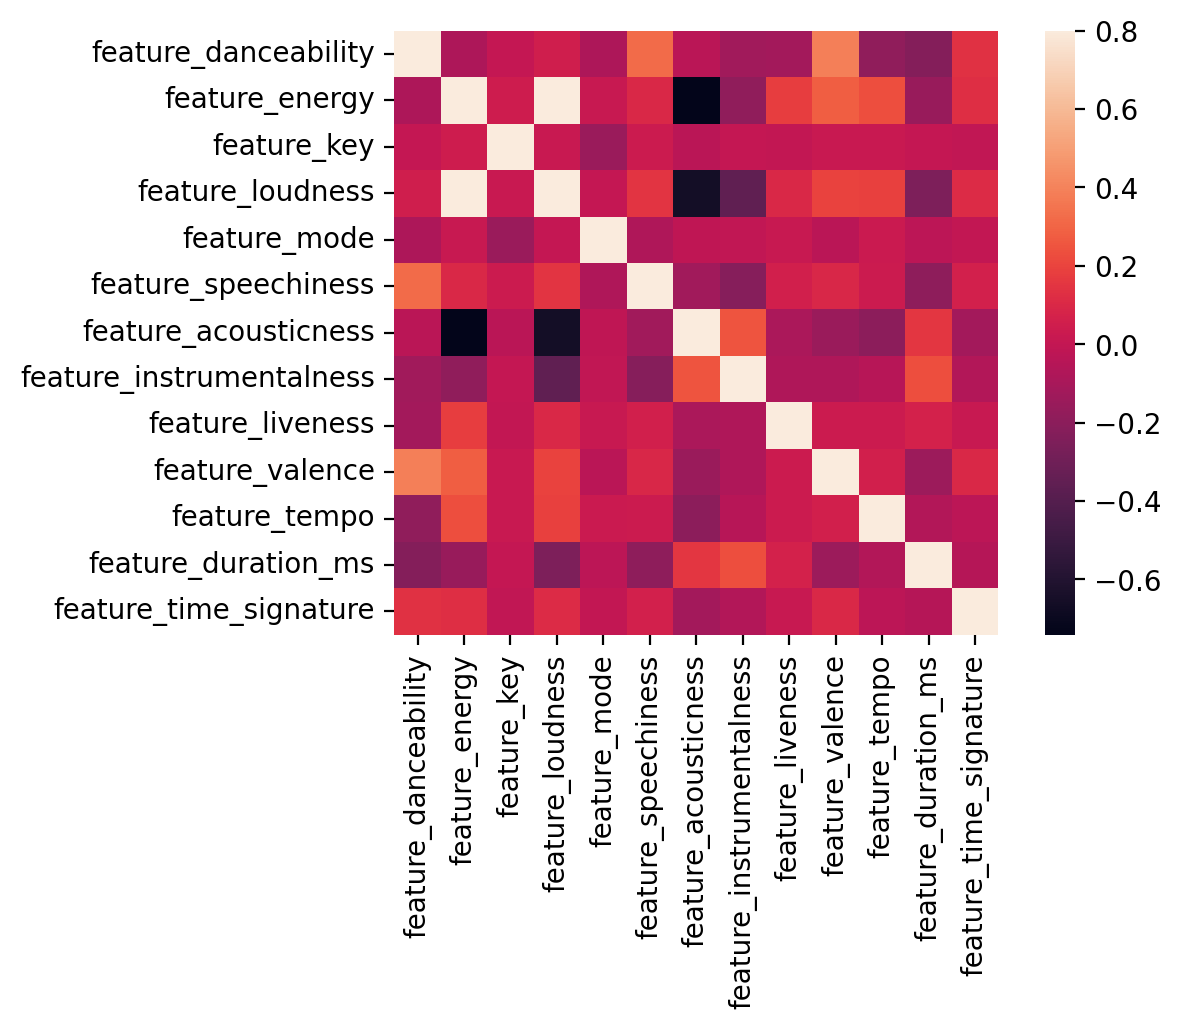
\includegraphics[width=0.6\textwidth]{overall_correlation}
\end{figure}

Generally, the features in the cluster "musical standards" can be ignored in this representation,
as they do not measure but only reflect characteristics (e.g., time signature or key).
It can be observed that \emph{energy} and \emph{loudness} have the highest correlation of the features,
with a value of approx. \(0.65\).  
This means that energetic songs have a tendency to also be loud.
The correlation matches the definition of these features as energetic tracks are defined to feel fast, loud, and noisy.
In addition, there is a comparatively high correlation between \emph{valence} and \emph{danceability} of
about \(0.5\), which means that positive songs encourage dancing.
The correlation between \emph{energy} and \emph{accousticness} is particularly negative, with a value of approximately \(-0.7\).
Acoustic tracks therefore often do not seem to be very energetic and vice versa.
The same can be said for \emph{accousticness} and \emph{loudness}, with a correlation value of about \(-0.5\).
Outside of these extreme values, the remaining correlation values settle between \(-0.2\) and \(0.2\).
Worth mentioning here are the correlations between \emph{instrumentalness} and \emph{loudness} at
approximately \(-0.3\) as well as \emph{instrumentalness} and \emph{valence} with around \(-0.3\).
Furthermore, a positive correlation between \emph{speechiness} and \emph{energy} can be observed at a value of around \(0.3\).

\begin{figure}[H]
    \centering
    \subfloat[\centering Correlation within \emph{rock}]{{\includegraphics[width=0.45\textwidth]{output_rock.png} }}%
    \qquad
    \subfloat[\centering Correlation within \emph{hiphop}]{{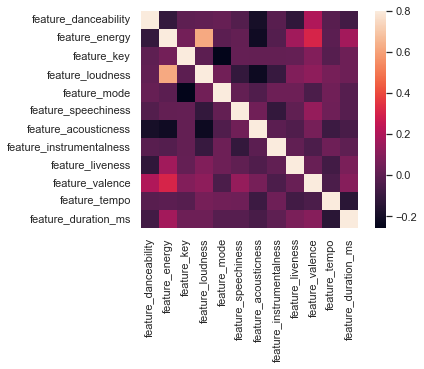
\includegraphics[width=0.45\textwidth]{output_Hip_Hop.png} }}%
    \qquad
    \subfloat[\centering Correlation within \emph{jazz}]{{\includegraphics[width=0.45\textwidth]{output_jazz.png} }}%
    \caption{Correlations within Categories}%
    \label{fig:du_cm_categorie_dependent}%
\end{figure}

The correlations in figure \ref{fig:du_cm_categorie_dependent} show the matrices on a per category basis.
The patterns described above can also be observed here.
However, the average correlation changes depending on the category.
For example, \emph{hiphop} shows the same characteristics as the category independent matrix but
the correlations are fundamentally more negative.

\subsubsection{Comparison of Music Theory to Audio Features}

An equally important step for data understanding is to compare features to the characteristics of genres
as described in music theory. Also a comparison between the categories itself is carried out.
This is necessary to develop a deeper understanding of the data.
As mentioned in the beginning of this chapter, theory and Spotify's findings are not always necessarily congruent,
which is why a clear delineation is important here.
% (e.g., "You can't dance well to \emph{rock}" - What is the overall value for Danceability?).
For this comparison, three features are chosen and discussed more deeply.
Subsequently, a better picture can be obtained with the help of further representations.

According to music theory a distinct property for rock songs is that they are very loud.
The characteristic is also present in the features created by Spotify in the feature \emph{loudness}
which is discussed here.
%In the category \emph{rock} one feature stands out: The songs are mostly loud.
%Overall, across all three categories, this feature has an average of -8.2544,
%with a minimum value of \(-32.06\) and a maximum value of \(2.044\).

\begin{figure}[H]
    \centering
    \subfloat[\centering Distribution Plot \emph{loudness}]{{\includegraphics[width=0.45\textwidth]{output_loudness.png} }}%
    \qquad
    \subfloat[\centering Boxplot \emph{loudness}]{{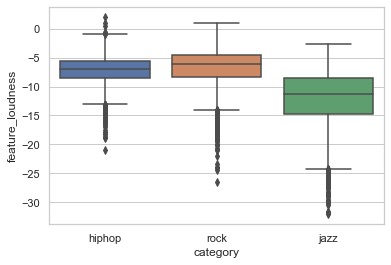
\includegraphics[width=0.45\textwidth]{output_Loudness_boxplot.png} }}%
    \caption{A Comparison of \emph{loudness} between the Categories}%
    \label{fig:du_dp_bp_ln_categorie_dependent}%
\end{figure}

Figure \ref{fig:du_dp_bp_ln_categorie_dependent}a shows a distribution plot.
The horizontal axis contains the value range of the feature \emph{loudness}.
The vertical axis shows the relative density of samples in a category at the respective loudness.
There are density curves for each of the categories, labeled accordingly.
Figure \ref{fig:du_dp_bp_ln_categorie_dependent}b shows a box plot, where the box represents values contained
between the 25th ($Q1$) and 75th ($Q2$) percentile and is called Interquartile Range ($IQR$).
The center line marks the median.
The lines outside of the box mark minimum ($Q1-1.5*IQR$) and maximum ($Q3+1.5*IQR$) values,
with the points outside of them representing outliers \cite{Galarnyk2018}.

These visualizations show, that \emph{hiphop} and \emph{rock} are more tightly distributed than \emph{jazz}.
\emph{jazz} spreads its songs over an area from \(-32.06\) to \(-2.695\) but locates
most songs at about \(-10\). \emph{hiphop} and \emph{rock} are distributed less widely and have 
a density which doubles that of \emph{jazz} at its highest point.
\emph{rock} places its point furthest to the right of the scale.
All of the features have a clear maximum density, which shows that a majority of tracks
are equally loud.
These observations confirm, that \emph{rock} is indeed the loudest category, closely followed by \emph{hiphop}.
This mimics the characteristics described in music theory.
\emph{jazz} can also have loud tracks, but the value range is far wider and it is generally more quiet.

The next feature discussed here is \emph{instrumentalness}.
Because the categories differ greatly in the amount of vocals used, differences can be expected here.
One would expect \emph{jazz} to have higher values, while vocals are an integral part of \emph{hiphop} 
and therefore the feature might be concentrated at lower value ranges.
The overall average for this feature is \(0.174\).
The lowest value overall is \(0.0\) while the highest goes up to \(0.989\).

\begin{figure}[H]
    \centering
    \subfloat[\centering Distribution Plot \emph{instrumentalness}]{{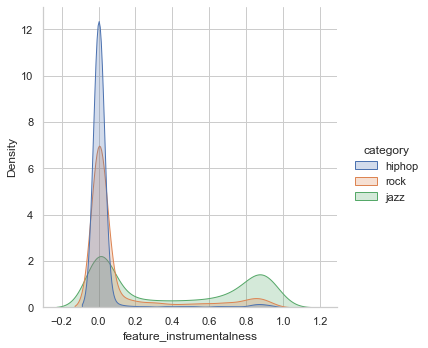
\includegraphics[width=0.45\textwidth]{output_instumentelness.png} }}%
    \qquad
    \subfloat[\centering Boxplot \emph{instrumentalness}]{{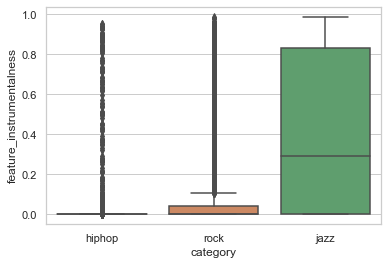
\includegraphics[width=0.45\textwidth]{output_instumentelness_boxplot.png} }}%
    \caption{A Comparison of \emph{instrumentalness} between the Categories}%
    \label{fig:du_dp_bp_instr_categorie_dependent}%
\end{figure}

Figure \ref{fig:du_dp_bp_instr_categorie_dependent} again shows a distribution plot and boxplot for \emph{instrumentalness}
It shows that both \emph{hiphop} and \emph{rock} are almost exclusively concentrated in the \(0.0\) to \(0.1\) range.
This means that almost all songs in these categories contain vocals.
However, slight increases in the range between \(0.8\) and \(1.0\) can also be seen.
\emph{jazz}, on the other hand, is grouped into two different maxima. One in the range around \(0.0\),
the other between \(0.8\) and \(1.0\). Since \emph{jazz} often contains only musical tracks without
any vocals, this reflects the reality quite well.
Here again, \emph{rock} and \emph{hiphop} are similar in their high points, while \emph{jazz} differs.
The distribution is more distributed and heterogeneous.

The last feature discussed in detail is \emph{energy}.
As explored in section \ref{sec:correlation between features} it correlates highly with the feature \emph{loudness}.
Therefore, one would expect similar results to the plots shown above.

\begin{figure}[H]
    \centering
    \subfloat[\centering Distribution Plot \emph{energy}]{{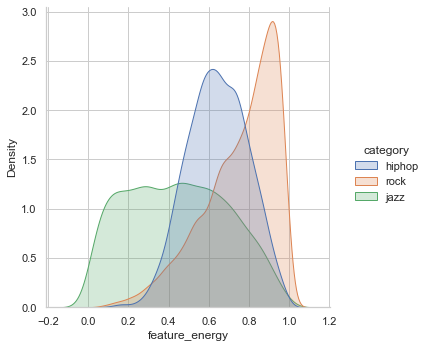
\includegraphics[width=0.45\textwidth]{output_energy.png} }}%
    \qquad
    \subfloat[\centering Boxplot \emph{energy}]{{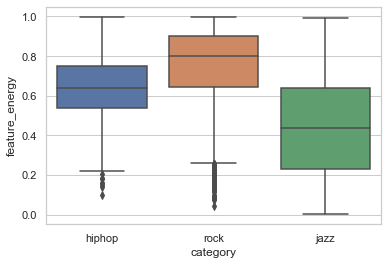
\includegraphics[width=0.45\textwidth]{output_energy_boxplot.png} }}%
    \caption{A comparison of \emph{energy} between the Categories}%
    \label{fig:du_dp_bp_enrg_categorie_dependent}%
\end{figure}

The plots (figure \ref{fig:du_dp_bp_enrg_categorie_dependent}) support the initial predictions, as \emph{rock} is again highly concentrated at the top of
the value range, followed by \emph{hiphop}. \emph{jazz} is again distributed very widely and
seems to generally be less energetic than the other categories. There is also not a clear maximum,
indicating that there does not seem to be a default energy level for \emph{jazz} artists.
Instead, artists seem to approach the genre from many different angles. This is seen in music
theory, as \emph{jazz} is divided into a number of subgenres with different properties.
In contrast to the distribution seen in \emph{loudness}, \emph{hiphop} is fairly broadly positioned.
It is a multi-faceted genre as well, which is supported by the data.

After these three sample features, additional Distribution- and Boxplots are visualized
to give further insights about the characteristics of the individual genres.

\begin{figure}[H]
    \centering
    \subfloat[\centering Distribution Plot \emph{Speechiness}]{{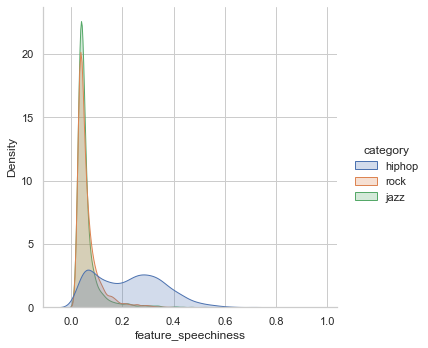
\includegraphics[width=0.4\textwidth]{output_Speechiness.png} }}%
    \qquad
    \subfloat[\centering Boxplot \emph{Speechiness}]{{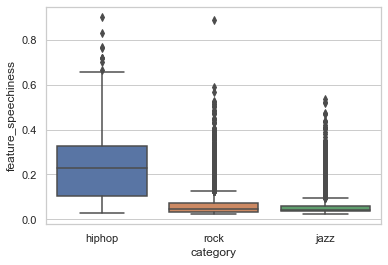
\includegraphics[width=0.4\textwidth]{output_Speechiness_Boxplot.png} }}%
    \qquad
    \subfloat[\centering Distribution Plot \emph{danceability}]{{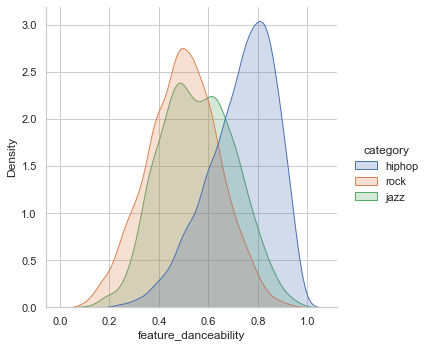
\includegraphics[width=0.4\textwidth]{output_Danceability.png} }}%
    \qquad
    \subfloat[\centering Boxplot \emph{danceability}]{{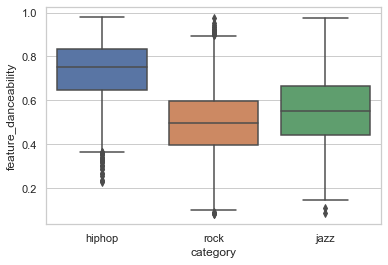
\includegraphics[width=0.4\textwidth]{output_Danceability_Boxplot.png} }}%
    \qquad
    \subfloat[\centering Distribution Plot \emph{accousticness}]{{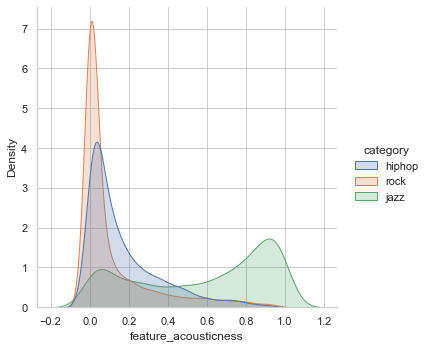
\includegraphics[width=0.4\textwidth]{output_accousticness.png} }}%
    \qquad
    \subfloat[\centering Boxplot \emph{accousticness}]{{\includegraphics[width=0.4\textwidth]{output_accousticness_Boxplot.png} }}%
    \qquad
    \subfloat[\centering Distribution Plot \emph{valence}]{{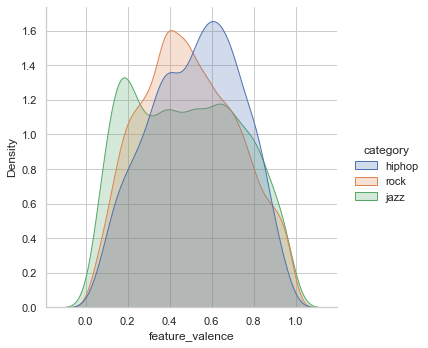
\includegraphics[width=0.4\textwidth]{output_valence.png} }}%
    \qquad
    \subfloat[\centering Boxplot \emph{valence}]{{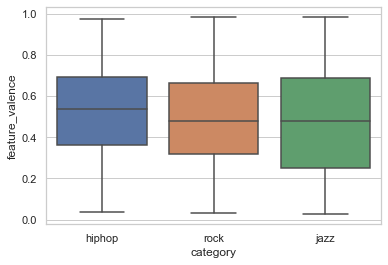
\includegraphics[width=0.4\textwidth]{output_valence_Boxplot.png} }}%
    \caption{Different Features visualized in Distribution- and Boxplots}%
    \label{fig:other exploration plots}%
\end{figure}